\documentclass{article}
\usepackage{listings}
\usepackage{color}
\usepackage{caption}
\usepackage{graphicx}
\usepackage{oz}
\DeclareGraphicsExtensions{.pdf,.png,.jpg}
\newtheorem{definition}{Definition}
 \usepackage{courier}
 \lstset{
         basicstyle=\footnotesize\ttfamily, % Standardschrift
         %numbers=left,               % Ort der Zeilennummern
         numberstyle=\tiny,          % Stil der Zeilennummern
         %stepnumber=2,               % Abstand zwischen den Zeilennummern
         numbersep=5pt,              % Abstand der Nummern zum Text
         tabsize=2,                  % Groesse von Tabs
         extendedchars=true,         %
         breaklines=true,            % Zeilen werden Umgebrochen
         keywordstyle=\color{red},
    		frame=b,         
 %        keywordstyle=[1]\textbf,    % Stil der Keywords
 %        keywordstyle=[2]\textbf,    %
 %        keywordstyle=[3]\textbf,    %
 %        keywordstyle=[4]\textbf,   \sqrt{\sqrt{}} %
         stringstyle=\color{white}\ttfamily, % Farbe der String
         showspaces=false,           % Leerzeichen anzeigen ?
         showtabs=false,             % Tabs anzeigen ?
         xleftmargin=17pt,
         framexleftmargin=17pt,
         framexrightmargin=5pt,
         framexbottommargin=4pt,
         %backgroundcolor=\color{lightgray},
         showstringspaces=false      % Leerzeichen in Strings anzeigen ?        
 }
 \lstloadlanguages{
         Java
 }
%\DeclareCaptionFont{blue}{\color{blue}} 

 %\captionsetup[lstlisting]{singlelinecheck=false, labelfont={blue}, textfont={blue}}
 % \usepackage{caption}
 
\DeclareCaptionFont{white}{\color{white}}
\DeclareCaptionFormat{listing}{\colorbox[cmyk]{0.43, 0.35, 0.35,0.01}{\parbox{\textwidth}{\hspace{15pt}#1#2#3}}}
 % \captionsetup[lstlisting]{format=listing,labelfont=white,textfont=white, singlelinecheck=false, margin=0pt, font={bf,footnotesize}}



\captionsetup[lstlisting]{format=listing,labelfont=white,textfont=white, singlelinecheck=false, margin=0pt, font={bf,footnotesize}}


\begin{document} 
\bgroup \parindent 0pt
{\Large\textbf{Model Catalogue - version2}}

\vskip 4mm 

{\Large {David Milward}}

\egroup

\vskip 14mm

\noindent

\section{Architecture}

The model catalogue version 2 is based on the existing model catalogue, but we are building it from scratch using the eclipse EMF model driven stack so that individual aspects of the model can be isolated and for academic reasons studied separately. As new designed elements are proved in the model catalogue 2 stack, we plan to adapt the existing Grails toolkit accordingly, but on an incremental basis.

The main classes in the metamodel are shown, together with their inheritance hierarchy in figure~\ref{fig:inheritance}. These are a \emph{CatalogueCore} class which roughly corresponding with the existing abstract \emph{CatalogueElement} class, it is intended to be an abstract class to which administrative behaviours can be added at a later stage, these will then be available in all the subclasses in the catalogue. We summarise these classes below:
\begin{itemize}
\item Catalogue Core - An abstract class allowing all other classes to be administered, annotated, constrained and associated.
\item DataModel - the main modelling artefact, all other entities will be a part of a DataModel
\item DataConcept - An abstract class which allows all its child classes to be treated as concepts.
\item DataSection - A grouping class for parts of a model, it can contain other DataSections, and DataClasses.
\item DataClass - A container for DataElements.
\item ValueDomain - A structure for the value/ representation of the DataElement.
\end{itemize}

 \begin{figure}[here]
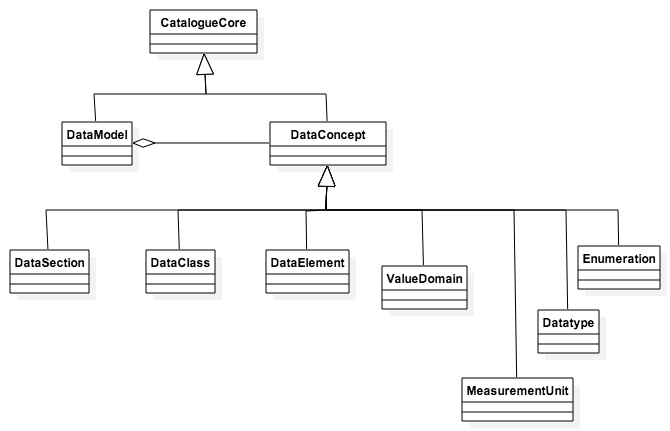
\includegraphics[scale=0.4]{images/inheritance}
\caption{Core Classes - Inheritance Model} 
\label{fig:inheritance}
\end{figure}

Figure~\ref{fig:core1} 



The \emph{CatalogueCore} class is the \emph{parent} of both the \emph{DataModel} and \emph{DataConcept} class, which are shown in figure~\ref{fig:core2} The \emph{DataModel} is a container class for all the models in the model catalogue, is roughly equivalent to the current \emph{Classification};  \emph{DataModels} will be the \emph{entities} that the model catalogue will manage.

 \begin{figure}[here]
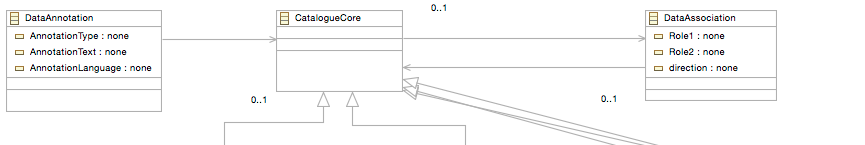
\includegraphics[scale=0.4]{images/core1}
\caption{Core Classes 1} 
\label{fig:core1}
\end{figure}

\subsection{Groupings inside the DataModel}

A \emph{DataAnnotation} class is needed to add annotations to any of the model elements in the model catalogue, and this can include constraints. We considered adding in a spearate constraint entity, however unless we are going to constraint the constraint to a particular language it seems acceptable to adopt the UML practise of including a constraint in an annotation. The annotation will have a type of either text or constraint (not shown yet ) and then it will have the annotation language, which depending on the type will either refer to a spoken language (such as German) or a constraint language (such as OCL).

\begin{figure}[here]
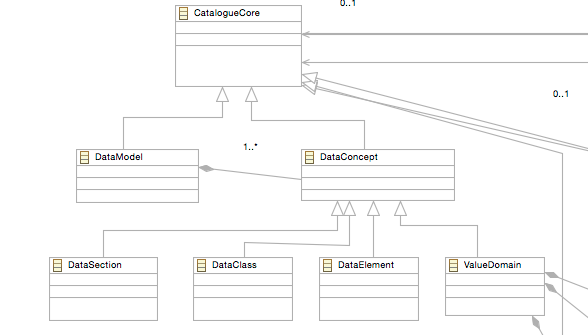
\includegraphics[scale=0.4]{images/core2}
\caption{Core Classes 2} 
\label{fig:core2}
\end{figure}

The class \emph{DataConcept} is an abstract class which is the parent of \emph{DataSection}, \emph{DataClass},\emph{DataElement}, \emph{ValueDomain}. The main idea behind having a single abstract parent class  \emph{DataConcept}  is to capture the notion that \emph{concepts} may be represented by any one of these classes within a model.  

The \emph{DataElement}, \emph{ValueDomain} are directly derived from the ISO11179 metadata registry standard, and correspond closely with the definitions provided within the standard. A data element in the current catalogue \emph{has} a single value domain, this is a one-to-one containment relationship. 

A \emph{DataClass} is simply a container for \emph{DataElements}, it's attributes are limited to \emph{DataElements}, and cannot be  \emph{DataClasses}. There is no upperbound on the number of \emph{DataElements} that can be contained in a \emph{DataClass}. Neither \emph{DataClass} nor \emph{DataElements} have an inheritance mechanism, although they can be associated using the \emph{DataAssociation} mechanism described earlier.

The \emph{DataSection} is a grouping element for \emph{DataElements} and \emph{DataClasses}, it corresponds to section in a documents and is needed as people will always section up large datasets into small digestible \emph{chunks}, normally these will be semantically related and stretch to about 7 entities. It seems sensible therefore to define a separate \emph{grouping} entities to enable this process. 

\subsection{Importing}

Importing can be carried out on any entity which is a child of the CatalogueCore entity, so that while whole DataModels can be imports, so too can DataSections, DataClasses, DataElements and ValueDomains. The standard package notation will apply, so that DataModel will be named using a name and a namespace (normally a URI), and this can be extended using dot notation, so that a DataModel will be identified by \textbf{DataModelName.example.org} and a section could be \textbf{DataSectionName.DataModelName.example.org}, and so forth.

An import will be a reference to an existing finalized DataModel, so that it will not be possible to change any entities within that imported DataModel. If the imported items need to be changed then the \emph{Cloning} operation is required.

\subsection{Cloning}

A clone will act in the same way as an import in terms of specifying the elements to be brought into the new DataModel, however these elements will be copied across as \emph{new and draft} elements into the new DataModel. They can therefore be changed and altered, they may retain an association with the old DataModel, however the association will be a \emph{basedon} type rather than \emph{is}. 



\subsection{Value Domains}

Value domains are entities which define how a \emph{DataElement} is represented in the underlying system, and to do this they can contain \emph{Datatypes}, \emph{Enumerations} and/or \emph{MeasurementUnits}. 

In the simplest example a \emph{DataElement} - say speed, can be represented by a \emph{ValueDomain} which has an integer \emph{Datatypes}. A  \emph{ValueDomain} entity being descended from a \emph{CatalogueCore} can then have a Constraint type of \emph{DataAnnotation} added which limits the speed to a value relative to the system under question, for boats perhaps a speed with an upper limit constraint of 600 (511 being the current world water speed record), and \emph{MeasurementUnits} of kph. 

The idea of a separate entity for measurement units is not completely neccessary as we could put that information into a \emph{DataAnnotation}.


\begin{figure}[here]
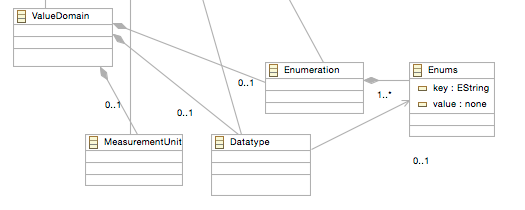
\includegraphics[scale=0.4]{images/core3}
\caption{Core Classes 3} 
\label{fig:core3}
\end{figure}





\end{document}